\documentclass{standalone}
\usepackage{tikz}
\usepackage{graphicx}
\usepackage{xcolor}
\usepackage{amsmath}

\newcommand{\jalrinstruction}[8]{
% Instruction are generally of 32 bits,
% so I will draw a box of length 32 and height 1,
% then I will insert the fields in such way:
% [imm[11:0] (12 bits) | rs1 (5 bits) | funct3 (3 bits) | rd (5 bits) | opcode (7 bits)] 
% I will draw vertical lines to separate the fields and then insert the text in the middle of the field 
% ps, in vim in order to set the tab size to 2 spaces, type :set tabstop=2 
\begin{scope}[shift={(#1, #2)}]
	\def\boxwidth{32}
	\def\height{1.5}
	\def\immwidth{12}
	\def\rsone{5}
	\def\functthree{3}
	\def\rd{5}
	\def\opcode{7}
	\draw[thick] (0, 0) rectangle (\boxwidth, -\height);
	\draw (\immwidth, 0) -- (\immwidth, -\height);
	\draw (\immwidth+\rsone, 0) -- (\immwidth+\rsone, -\height);
	\draw (\immwidth+\rsone+\functthree, 0) -- (\immwidth+\rsone+\functthree, -\height);
	\draw (\immwidth+\rsone+\functthree+\rd, 0) -- (\immwidth+\rsone+\functthree+\rd, -\height);
	\node[anchor=mid, align=center] at (\immwidth/2, -\height/2) {\LARGE \textbf{#3}};
	\node[anchor=mid, align=center] at (\immwidth+\rsone/2, -\height/2) {\LARGE \textbf{#4}};
	\node[anchor=mid, align=center] at (\immwidth+\rsone+\functthree/2, -\height/2) {\LARGE \textbf{#5}};
	\node[anchor=mid, align=center] at (\immwidth+\rsone+\functthree+\rd/2, -\height/2) {\LARGE \textbf{#6}};
	\node[anchor=mid, align=center] at (\immwidth+\rsone+\functthree+\rd+\opcode/2, -\height/2) {\LARGE \textbf{#7}};
	\node[anchor=mid, anchor=north, 
	  align=center, text width=23cm, 
	  font=\LARGE,
	  inner sep=0pt] at (16, -2) {#8};
\end{scope}
}

\begin{document}
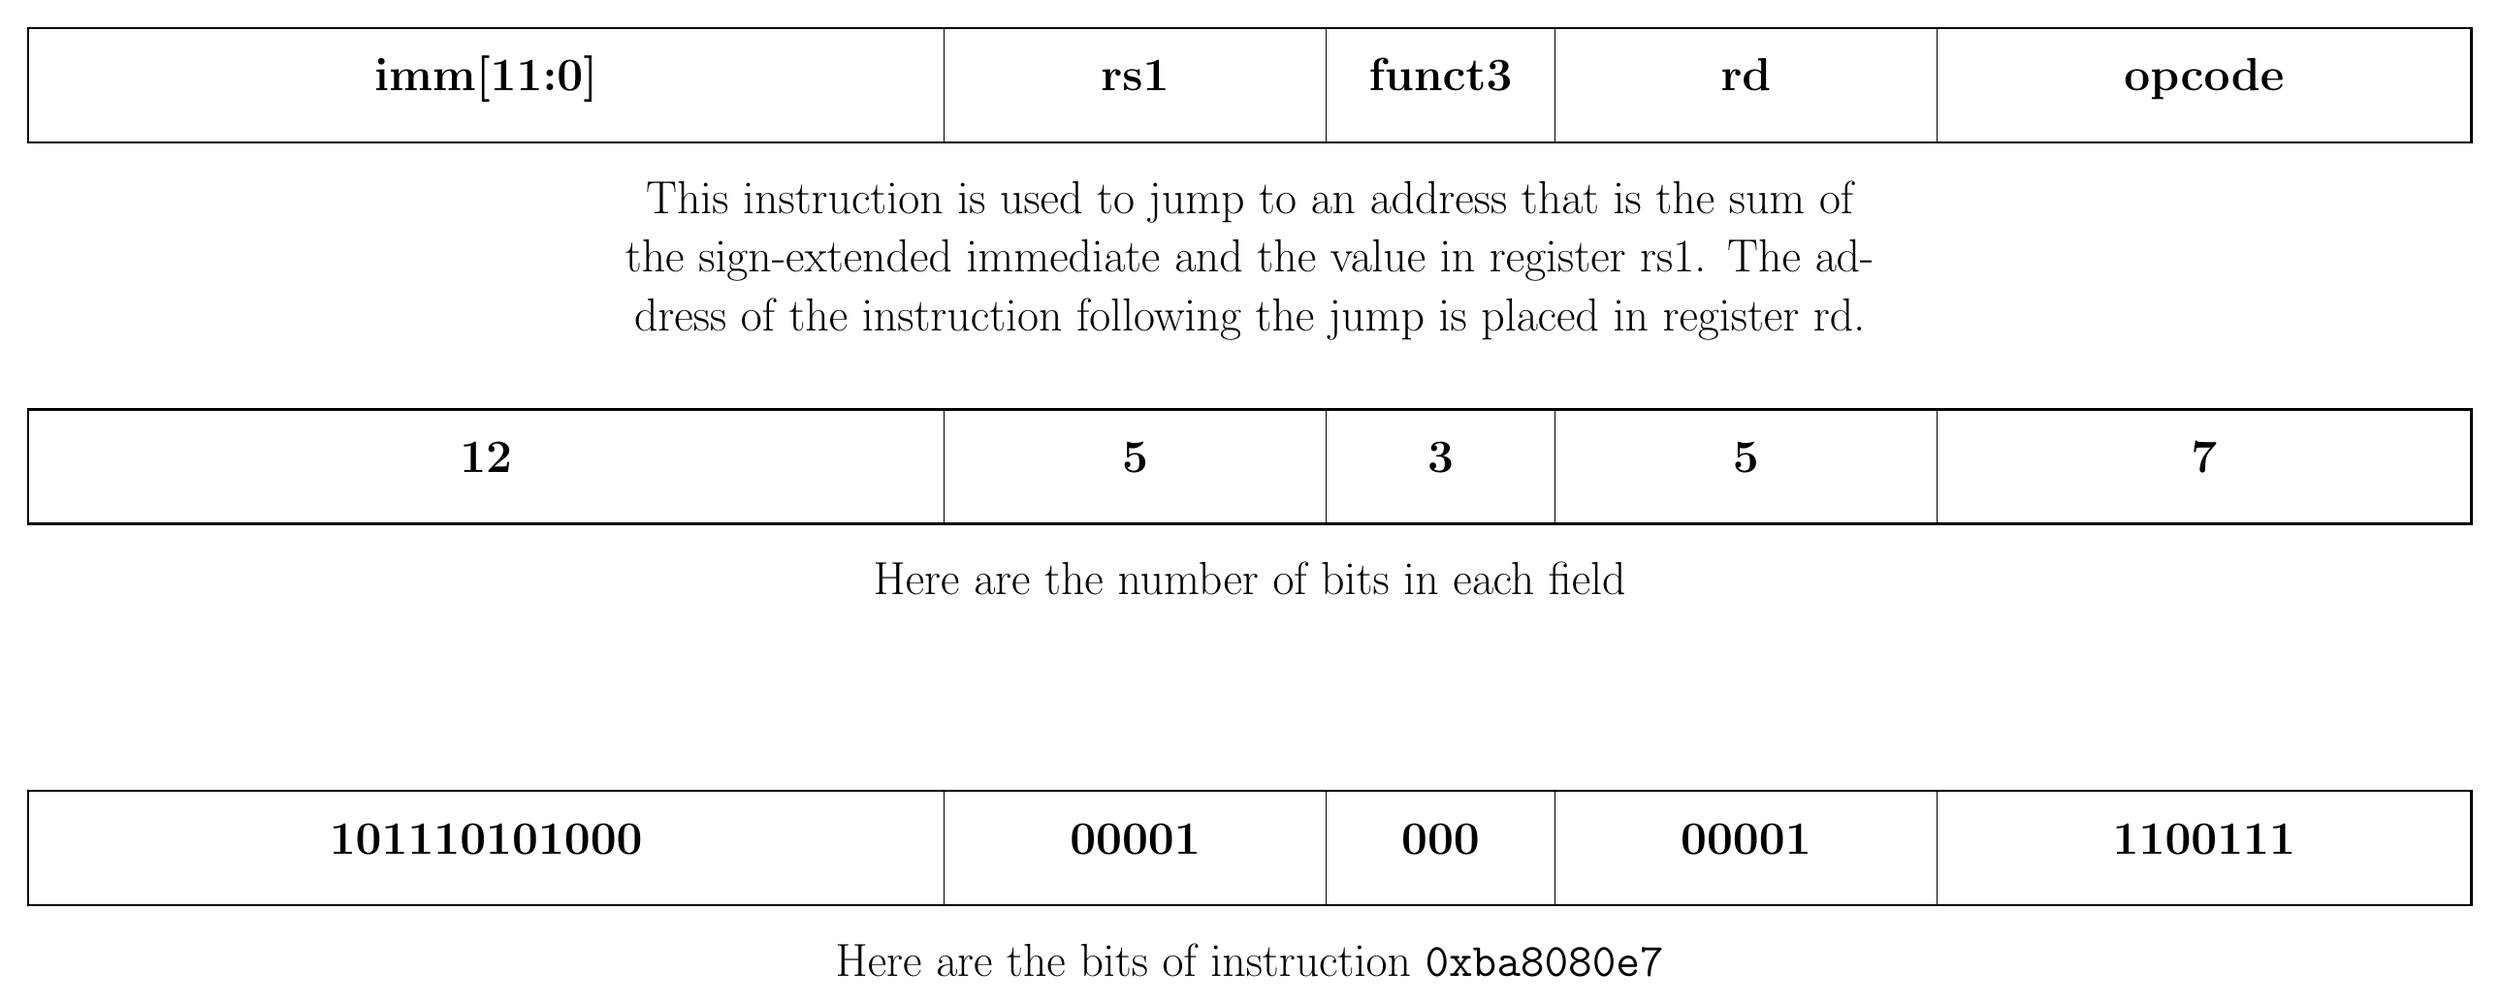
\begin{tikzpicture}
\def\descjalr{
This instruction is used to jump to an address that is the sum of the sign-extended immediate and the value in register rs1. The address of the instruction following the jump is placed in register rd. 
}

\jalrinstruction{0}{0}{imm[11:0]}{rs1}{funct3}{rd}{opcode}{\descjalr}

\jalrinstruction{0}{-5}{12}{5}{3}{5}{7}{Here are the number of bits in each field}

\jalrinstruction{0}{-10}{101110101000}{00001}{000}{00001}{1100111}{Here are the bits of instruction \texttt{0xba8080e7}}

\end{tikzpicture}
\end{document}
